
\documentclass[11pt,a4paper]{article}
\usepackage[utf8]{inputenc}
\usepackage{amsmath, amssymb, amsthm}
\usepackage{geometry}
\usepackage{graphicx} % Include graphics
\usepackage{hyperref} % Hyperlinks
\usepackage{enumerate} % Customizable enumeration
\geometry{a4paper, margin=1in}

\theoremstyle{plain}
\newtheorem{theorem}{Theorem}[section]
\newtheorem{lemma}[theorem]{Lemma}
\newtheorem{proposition}[theorem]{Proposition}
\newtheorem{corollary}[theorem]{Corollary}
\theoremstyle{definition}
\newtheorem{definition}[theorem]{Definition}
\newtheorem{example}[theorem]{Example}
\newtheorem*{definition*}{Definition}
\theoremstyle{remark}
\newtheorem*{remark}{Remark}
\newtheorem*{note}{Note}

\begin{document}

% \tableofcontents

\chapter{Chapter 1}

\section{Curse of Dimensionality and Neural Networks}

We approach this chapter knowing the following
\begin{itemize}
    \item \textbf{Universal approximation theorem}: Both shallow and deep networks are universal, that is they can approximate arbitrarily well any continuous function of \(n\)  variables on a compact domain. \cite{UniversalApprox}.
    
    This is a classical result for shallow networks, and the same result holds for deep networks. Since \(\{\text{Shallow Networks}\} \subseteq \{\text{Deep Networks}\}\), there too exists deep networks that can approximate any continuous function of \(n\) variables on a compact domain arbitrarily well.

    \item \textbf{Deep networks can beat the curse}: Theory on shallow networks is well understood and dates well back to at least the 1980s. However, the theory on deep networks is less well understood, for a review we can refer to \cite{DeepReviewNature}. Within this review we see results on how deep convolutional nets and recurrent nets have been able to beat the curse, in tasks such as image processing and speech recognition. We see that deep learning outperforms traditional machine-learning methods by automatically discovering intricate structures in high-dimensional data. Perhaps by use of hierarchical architectures, deep networks can exploit some form of structure in the data to beat the curse.
    
    \item \textbf{\textit{"Are hierarchical architectures with more layers justifiable in terms of learning theory?"}} \cite{poggioHierarchy}
    
    We find that in many cases in past works, little attention was given to multi-layer networks as often shallow nets performed empirically as well \cite{what}. However, \cite{poggioHierarchy} motivates a strong question regarding hierarchies; \textit{"It seems that the learning theory of the type we have outlined does not offer any general argument in favor of hierarchical learning machines for regression or classification. This is somewhat of a puzzle since the organization of cortex - for instance visual cortex - is strongly hierarchical. At the same time, hierarchical learning systems show superior performance in several engineering applications.”}. So there are occasions where deep networks can outperform shallow networks, and we would expect this to be the case by comparison to a neural network we already see in nature - the human brain. The question is now, that if we know such deep networks exist and can outperform shallow networks, can we justify this in terms of learning theory, and how do we construct them?
\end{itemize}

\subsection{Shallow and Deep Networks}

\begin{definition}[Shallow Neural Network (Single Hidden Layer)]

A shallow neural network with a single hidden layer is defined by the following components:

\begin{itemize}
  \item \textbf{Input Layer:} Let \(\mathbf{x} = (x_1, x_2, \ldots, x_d)^T\) represent the input vector where \(d\) denotes the number of input features/dimensions, thus \(\mathbf{x} \in \mathbb{R}^d\).

  \item \textbf{Hidden Layer:} The hidden layer consists of \(h\) neurons. Each neuron \(j\) applies a transformation to the input vector, characterized by a weight vector \(\mathbf{w}_j \in \mathbb{R}^d\) and a scalar bias \(b_j\). The activation function \(\sigma\) is applied to the linear combination of the inputs:
    \[
    z_j = \sigma(\mathbf{w}_j^T \mathbf{x} + b_j)
    \]
    The output of the hidden layer can be expressed as \(\mathbf{z} = (z_1, z_2, \ldots, z_h)^T \in \mathbb{R}^h\).

  \item \textbf{Output Layer:} Assuming a single output neuron, the final output \(y\) of the network is produced by applying another activation function \(\phi\) to the linear combination of the hidden layer outputs:
    \[
    y = \phi(\mathbf{v}^T \mathbf{z} + c)
    \]
    where \(\mathbf{v} \in \mathbb{R}^h\) and \(c\) is a scalar bias.
\end{itemize}
\end{definition}


\begin{definition}[Deep Neural Network]

A \textbf{deep neural network} is a function \( f: \mathbb{R}^n \rightarrow \mathbb{R}^m \) constructed by a sequence of compositions of simpler functions, each representing a layer in the network. The architecture of a deep neural network can be described by a directed acyclic graph (DAG), denoted as \( G = (V, E) \), where:

\begin{itemize}
    \item \( V \) represents the set of vertices, with each vertex corresponding to a layer in the network.
    \item \( E \) represents the set of edges, where each directed edge \( (u, v) \in E \) indicates that the output of layer \( u \) is the input to layer \( v \).
\end{itemize}

Each vertex \( v \in V \) in the graph is associated with a transformation function \( f_v: \mathbb{R}^{n_v} \rightarrow \mathbb{R}^{m_v} \) and is characterized by the following components:

\begin{enumerate}
    \item \textbf{Neurons}: Each layer \( v \) consists of \( m_v \) neurons. The number of neurons \( m_v \) in each layer can vary depending on the layer's role and design within the network.
    \item \textbf{Activation Function}: Each layer includes an activation function \( \sigma_v: \mathbb{R}^{m_v} \rightarrow \mathbb{R}^{m_v} \), which introduces non-linearities into the network, enabling it to model complex relationships.
    \item \textbf{Weights and Biases}: Each connection \( (u, v) \in E \) is characterized by a weight matrix \( W_{uv} \in \mathbb{R}^{m_u \times n_v} \) and a bias vector \( b_{uv} \in \mathbb{R}^{n_v} \), which are parameters that are learned during training.
\end{enumerate}

The output of each layer \( v \) is given by:
\[
y_v = \sigma_v(W_{uv} y_u + b_{uv})
\]
where \( y_u \) is the output from the previous layer \( u \). For the initial layer \( v_0 \) in the graph, the input \( x \in \mathbb{R}^n \) is used:
\[
y_{v_0} = \sigma_{v_0}(W_{v_0} x + b_{v_0})
\]

The overall output of the network \( f(x) \) is the output of the final layer in the topology of \( G \).

\end{definition}

\begin{figure}[h!]
    \centering
    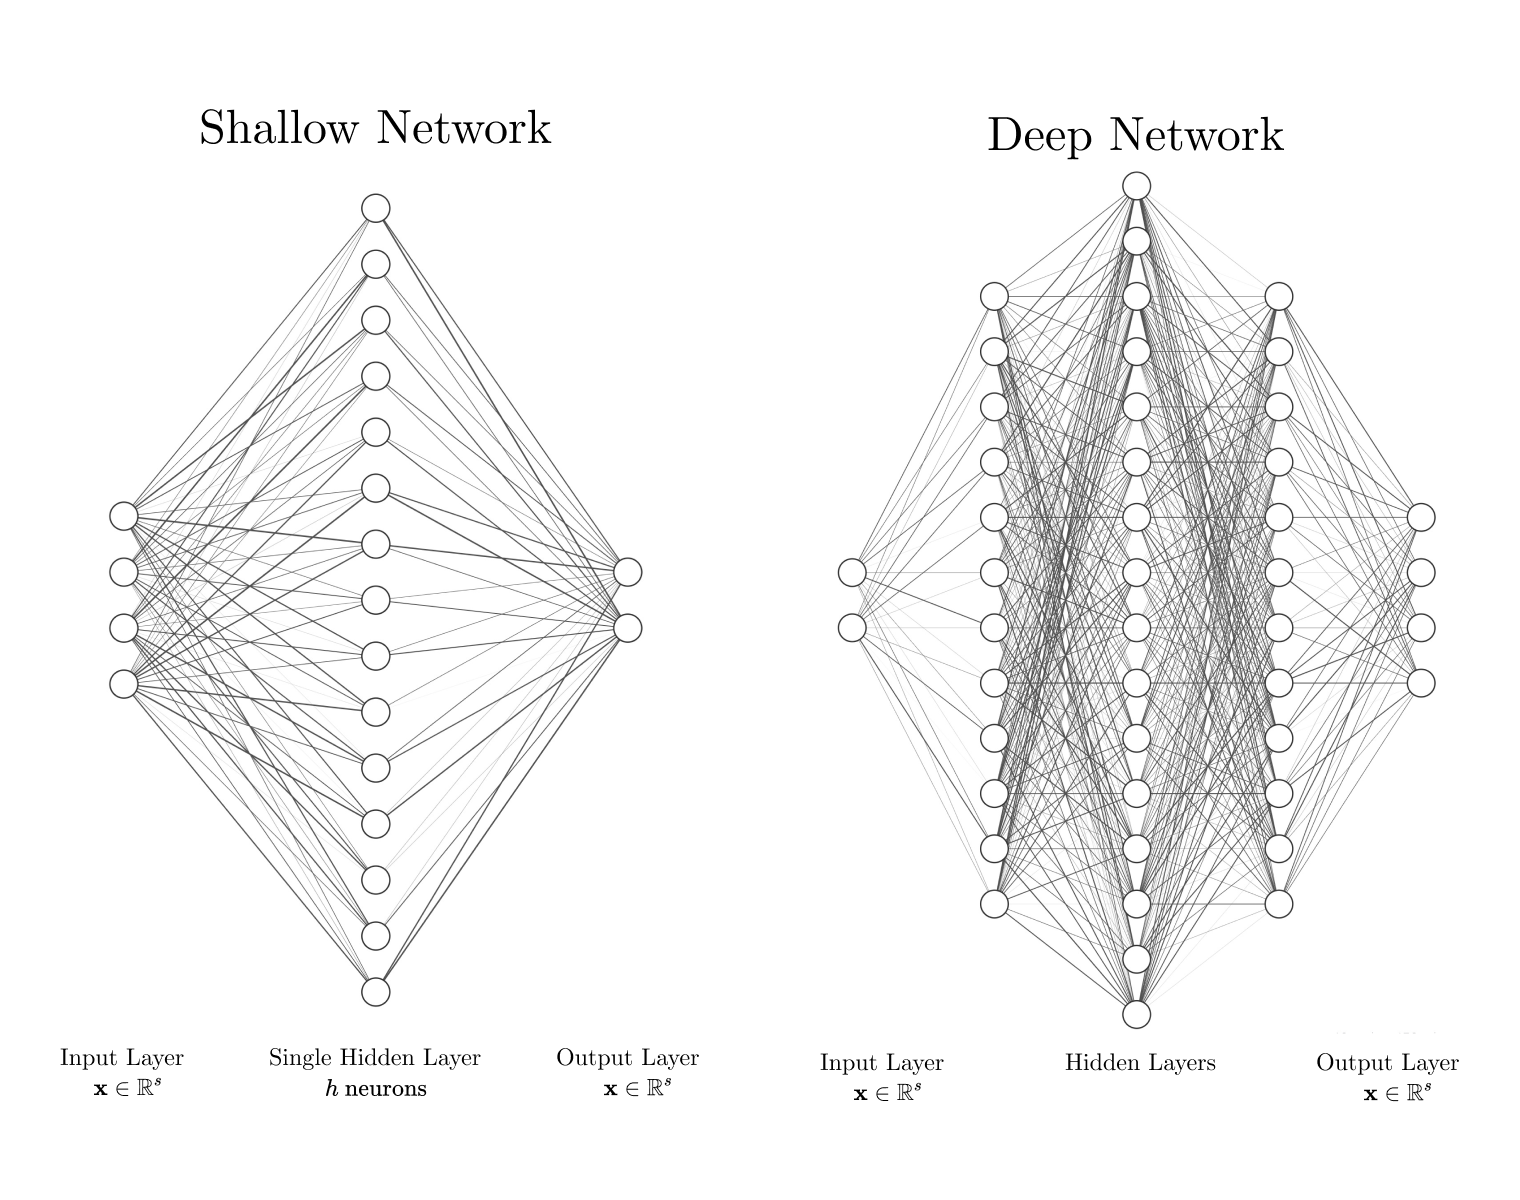
\includegraphics[width=0.8\textwidth]{diags/shallow_deep.png}
\end{figure}

\subsection{Examples of Deep Networks beating the curse}

Deep neural networks have been applied successfully to a range of problems that involve high-dimensional data, showcasing their ability to beat the curse of dimensionality. Here are a few prominent examples:

\begin{itemize}
    \item ResNet-152: A deep residual network with 152 layers, which has been shown to achieve state-of-the-art performance on the ImageNet dataset. \cite{ResNet}

    \item \textbf{Image Recognition}: In the realm of image recognition, Convolutional Neural Networks (CNNs) have become the standard. High-dimensional image data, which can include millions of pixels, is effectively managed by CNNs through hierarchical feature extraction and weight sharing. A landmark moment was when AlexNet dramatically improved performance on the ImageNet challenge, processing images with high resolution to accurately classify them into thousands of categories.
    
    \item \textbf{Natural Language Processing (NLP)}: Models like BERT (Bidirectional Encoder Representations from Transformers) and GPT (Generative Pre-trained Transformer) handle the high dimensionality of linguistic data, which includes extensive vocabularies and diverse syntactic structures. These models use attention mechanisms and embeddings to reduce dimensionality and capture semantic relationships within text, enabling them to excel in tasks like translation, text summarization, and sentiment analysis.
    
    \item \textbf{Speech Recognition}: Deep neural networks, specifically deep belief networks (DBNs) and recurrent neural networks (RNNs), have significantly improved the performance of speech recognition systems. These networks process raw audio data, which is inherently high-dimensional, to extract features and recognize speech patterns over time, even in noisy environments.
    
    \item \textbf{Medical Imaging}: Deep learning has also made substantial impacts in the analysis of medical images, such as MRI scans and CT scans, which are high-dimensional. Networks like U-Net have been specifically designed for biomedical image segmentation, efficiently processing these images to detect, for example, tumor boundaries against the backdrop of normal anatomical structures.
    
    \item \textbf{Financial Time Series Forecasting}: Despite the challenges posed by the noisy and non-stationary nature of financial markets, deep learning models like Long Short-Term Memory networks (LSTMs) have been used to forecast market movements based on high-dimensional input features, including historical price data, volume, and macroeconomic indicators.
    
    \item \textbf{Autonomous Vehicles}: The perception systems of autonomous vehicles are another area where deep neural networks manage high-dimensional sensory inputs, including LIDAR, radar, and video. These systems must process and interpret vast amounts of data in real-time to make driving decisions, an application where CNNs and RNNs have proven particularly effective.

\end{itemize}

These examples demonstrate how deep neural networks can effectively manage and exploit high-dimensional data across different domains, providing solutions where traditional methods fall short.

\subsection{Why Sobolev Spaces?}

In theoretical investigations of the degree of approximation, one typically makes an a priori assumption that the target function \(f\), although itself unknown, belongs to some known class of functions.

In this report, we are interested in the Sobolev classes. By assuming our target function belongs to some smoothness class, we are enabled to make comments on the required complexity of a network to achieve a desired accuracy. This assumption is what gives us the theoretical guarantees we seek.

We can also leverage these assumptions in the training process, where we have seen Sobolev training in action already in the literature. \cite{sobolevtraining}, making use of more data than just input-output data pairs to train a network. We explore this later.

Our main method of improving upon the efficiency of a shallow network by use of deep networks will be via architecture solutions - assumptions on the smoothness and compositionality of the target function will be key in this process.

\subsection{Main theorems}

This section focuses on the results from Poggio, T. and Liao, Q. (2018) 'Theory I: Deep networks and the curse of dimensionality'. \cite{poggio}.

We take \(\Pi_{n}\) to denote the set all neural networks with complexity \(n\), taken here as the total number of units in the network (e.g. shallow networks of \(n\) neurons in its hidden layer). Trivially we have \(\Pi_{n} \subseteq \Pi_{n+1} \).
We measure the degree of approximation error as:

\[
    \text{dist} (f  - \Pi_{n}) = \inf_{g \in \Pi_{n}} \left\| f - g \right\|
\]

The norm more classically associated for measuring the performance of a neural network is the \(L^2\) norm, however the \textit{sup} norm is used here to provide a stronger condition for the approximation error.

Note that if \(dist(f, \Pi_{n}) = \mathcal{O}(n^{-\gamma} )\), for some \(\gamma > 0\)  then a network of complexity \(n = \mathcal{O}(\epsilon^{-\frac{1}{\gamma }}) \) can guarantee an approximation error of at least \(\epsilon \).

Within this paper, the authors state two theorems, which are as follows:

\begin{enumerate}
    
\item \textbf{Theorem 1}: (Shallow Networks)

It states that for a function \( f \in W_{m}^{n} \), the set of all functions of \(n\) variables with continuous partial derivatives up to order \(m < \infty \) such that \(\left\lVert f\right\rVert + \sum_{1\leq \left\vert \mathbf{k}  \right\vert_{1} \leq m} \left\lVert \mathbf{D}^{k} f\right\rVert \leq 1  \), and an activation function \( \sigma: \mathbb{R} \rightarrow \mathbb{R} \) that is infinitely differentiable and not a polynomial, the complexity of shallow networks that provide accuracy at least \( \varepsilon \) is 
\[ N = O(\varepsilon^{-n/m}) \]

\item \textbf{Theorem 2}: (Deep Networks - Binary Tree)

It considers a function \( f \in W_{m}^{2,n} \), the class of all compositional functions \(f\) of \(n\) variables with a binary tree architecture and constituent functions \(h\)  in \(W_{m}^{2}\)  and a deep network with a compositional architecture.\\
The activation function \( \sigma: \mathbb{R} \rightarrow \mathbb{R} \) in this context is also infinitely differentiable and not a polynomial. The complexity of the network necessary to provide an approximation with accuracy at least \( \varepsilon \) is 

\[ N = O((n - 1)\varepsilon^{-2/m}) \]
\end{enumerate}

\begin{figure}[h]
    \centering
    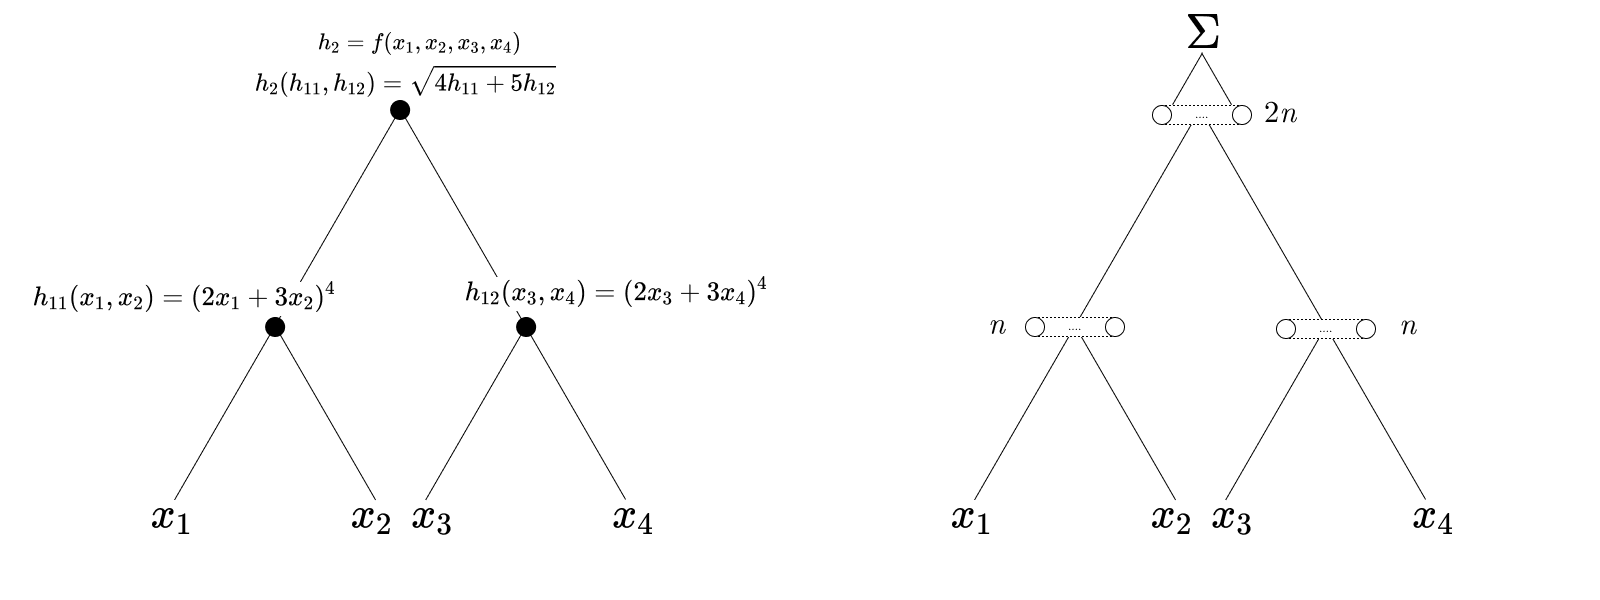
\includegraphics[width=\textwidth]{diags/BinaryTree.png}
    \caption{Binary Tree Architecture}
    \label{fig:}
\end{figure}



\subsection{Spaces \& Norms}
We first take care to mention the spaces and norms we are using. If we intend to measure the quality of an approximation, we must carefully consider how to do this and how the use of various norms interact with one another, and what that implicates for our results. In particular we use 2 types of norms:

\subsubsection{The \( L^p \)-norm (\( \|\cdot\|_p \))}

This norm is used to measure the approximation error between the function \( f \) and our approximation.

If \( A \subseteq R^{s}\) is Lebesgue measurable, and \(f : A \to R\) is a measurable function, we define the \(L^{p} (A)\) norms of \(f\) as follows:   
   \[
   \|f\|_{p,A} = 
   \begin{cases} 
   \left( \int_{A} |f(x)|^p dx \right)^{1/p}, & \text{for } 1 \leq p < \infty, \\
   \text{ess sup}_{x \in A} |f(x)|, & \text{for } p = \infty.
   \end{cases}
   \]


   The class of all functions such that \(\left\lVert f\right\rVert_{p,A} < \infty \) is denoted by \(L^p(A)\) 

   Take \(L^{\infty }(A)\) as the space of continuous functions on \(A\).

   Throughout this report we take \(A = [-1,1]^s\), unless explicitly stated otherwise.

   

\subsubsection{Sobolev Norm \((\|\cdot\|_{W^p_{r,s}})\) }

We first define the space as follows: 

Let \(r \geq 1\) an integer and \(Q\) a cube in \(\mathbb{R}^{s}\). The class \(W^p_{r,s}(Q)\) consists of all functions with \(r - 1\) continuous partial derivatives on \(Q\) which in turn can be expressed (almost everywhere on \(Q\)) as indefinite integrals of functions in \(L^p(Q)\). Alternatively, the class \(W^p_{r,s}(Q)\) consists of functions which have, at almost all points of \(Q\), all partial derivatives up to order \(r\) such that all of these derivatives are in \(L^p(Q)\). 

The Sobolev norm of \(f \in W^p_{r,s}(Q)\) is defined by 

\[
\|f\|_{W^p_{r,s}(Q)} = \sum_{0\leq |k| \leq r}  \left\lVert D^{\mathbf{k}} f\right\rVert_{p,Q}   
\]

where for the multi-integer \( \mathbf{k}  = (k_1,...,k_s) \in \mathbb{Z}^s \), \( 0 \leq \mathbf{k}  \leq r \) means that each component of \( \mathbf{k}  \) is nonnegative and does not exceed \( r \), \( |\mathbf{k} | := \sum_{j=1}^{s} |k_j| \) and 

\[
    D^{\mathbf{k} }f = \frac{\partial^{|\mathbf{k} |} f}{\partial x_1^{k_1} \cdots \partial x_s^{k_s}}, \quad k \geq 0
\]

Again \(W^{\infty }_{r,s}(Q)\) will denote the class of functions which have continuous derivatives of order \(r\) and lower. As before, if \(Q = [-1, 1]^s\), we will not mention it in the notation. Thus, we write \(W^p_{r,s} = W^p_{r,s}([-1, 1]^s)\) etc.

\section{Theorem 1}

We state the theorem and proof from \cite{Mhaskar} as follows;

Let $1 \leq d \leq s, n \geq 1$ be integers, $f : \mathbb{R}^s \rightarrow \mathbb{R}$ and $\phi : \mathbb{R}^d \rightarrow \mathbb{R}$. A \textit{generalized translation network} with $n$ neurons evaluates a function of the form $\sum_{k=1}^n a_k \phi(A_k (\cdot) + \mathbf{b}_k)$ where the \textit{weights} $A_k$s are $d \times s$ real matrices, the \textit{thresholds} $\mathbf{b}_k \in \mathbb{R}^d$ and the \textit{coefficients} $a_k \in \mathbb{R}$ $(1 \leq k \leq n)$. The set of all such functions (with a fixed $n$) will be denoted by $\Pi_{\phi;n,s}$.

We attempt to approximate \(f\) by elements of \(\Pi_{\phi;n,s}\) on the domain \([-1,1]^s\). For the \(d=1\) case we have \(\Pi_{\phi;n,s} \) simply the collection of shallow networks with \(n\) neurons in their hidden layer.

This construction will not provide the best approximation, but will instead provide the optimal order of approximation. We have also, that the weights \(A_{k}\)'s and the thresholds \(\mathbf{b}_{k}\)'s  will be determined independently of the target function
\(f\).

We observe a notable assumption that we are able to sample from the
target function at all prescribed points without noise.




\subsection{Statement}


We can make the following statement for the required complexity of a shallow network to approximate a function in a Sobolev space.\\

Let \(1 \leq d \leq s\), \(r \geq 1\), \(n \geq 1\) be integers and \(1 \leq p \leq \infty\). Let \(\phi: \mathbb{R}^d \rightarrow \mathbb{R}\) be infinitely many times continuously differentiable in some open sphere in \(\mathbb{R}^d\). It is further assumed that there exists a point \(b\) in this sphere such that

\begin{equation}
    D^k \phi(b) \neq 0, \mathbf{k} \in \mathbb{Z}^d, \mathbf{k} \geq 0
    \label{derCondition}
\end{equation}

Note that the above condition, is equivalent to the statement that the function \(\phi\) is not a polynomial. This is shown in \cite{25Poggio}.

Then, there exist \(d \times s\) matrices \(\{A_j\}_{j=1}^n\) with the following property: For any function \(f\) in the Sobolev space \(W^p_{r,s}\), there exist coefficients \(a_j(f)\) such that

\begin{equation}
    \left\| f - \sum_{j=1}^{n} a_j(f) \phi(A_j(\cdot) + b_{j}) \right\|_p \leq c n^{-r/s} \|f\|_{W^{p}_{r,s}}
\end{equation}

Here, the functionals \(a_j\) are continuous linear functionals on \(W^p_{r,s}\).

In particular, we measure the \textit{degree of approximation} of \(f\) by the expression

   \[
    E_{\phi;n,p} = \inf\{ \left\| f - g \right\|_p : g \in \Pi_{\phi ; n,s} \}
   \]

   The quantity \(E_{\phi ; n,p}\)  denotes the theoretically minimal error that can be achieved in approximating the function \(f\)  in the \(L^p\)  norm by generalized translation networks with \(n\)  neurons each evaluating the activation function \(\phi \).

\[ E_{\phi ; n,p,r,s} := \sup\{E_{\phi ; n,p}(f) : \|f\|_{W^p_{r,s}} \leq 1\}  \leq c n^{-r/s} \]

where \( E_{\phi;n,r,s,p} \) denotes the maximal error that can be achieved in approximating functions in \(W^p_{r,s}\) by generalized translation networks with \(n\) neurons each evaluating the activation function \(\phi \), with the assumption that the target function \(f \in W^p_{r,s}\) is properly normalised. Here we take the fact that that any function in \(W^p_{r,s}\) can be normalized so that \( \|f\|_{W^p_{r,s}} \leq 1 \).

\subsection{Proof} 

\subsubsection{Idea for Proof}

For every integer \(m \geq r, \exists \) polynomial \(P_{m}(f)\) of co-ordinatewise degree not exceeding \(m\) such that \(\forall f \in W^{p}_{r,s}\).

\[
\|f - P_{m}(f)\|_{p,[-\pi,\pi]^s} \leq \frac{c}{m^r} \|f\|_{W^{p*}_{r,s}}  
\]

(By co-ordinatewise degree, we mean that the degree of the polynomial in each variable is at most \(m\)). Aim to express each monomial in \(P_{m}(f)\) with suitable derivative of \(\phi \), then take each derivative approximations and approximate it by an appropriate divided difference method involving \(O(m^s)\) evaluations of \(\phi \) 

\subsubsection{Useful Definitions and clarifications}


\begin{itemize}
    \item \(\left\vert \mathbf{k}  \right\vert = \sum_{j} k_{j}\)
    \item  \(0 \leq \mathbf{k} \leq \mathbf{r}  \iff 0 \leq k_{j}\leq r_{j} \forall j\) 
    \item \(L^{p^{\ast} } := L^{p}([-\pi ,\pi ]^s) \), \(W^{p^{\ast} }_{r,s} := W^{p}_{r,s} ([-\pi ,\pi ]^s)\) 

    \item \textbf{Fourier Coefficients}: For a function \( g \in L^{p^*} = L^{p}([-\pi ,\pi ]^s) \), its Fourier coefficients are given by the following, where \( \mathbf{k} \) is a multi-index in \( \mathbb{Z}^s \), and \( \mathbf{t}  \) is in the domain \( [-\pi, \pi]^s \).

    \begin{equation}
        {g}(\mathbf{k}) := \frac{1}{(2\pi)^s} \int_{[-\pi,\pi]^s} g(\mathbf{t})e^{-i \mathbf{kt}} d \mathbf{t}, \quad \mathbf{k} \in \mathbb{Z}^s.  
    \end{equation}


    \item \textbf{Partial Sums of the Fourier Series}: The partial sum \( s_m(g, t) \) of the Fourier series of \( g \) is given as follows,
    
    \begin{equation}
        s_m(g(\mathbf{k}),t) := \sum_{-\mathbf{m} \leq \mathbf{k} < \mathbf{m}}  {g}(\mathbf{k})e^{i \mathbf{kt}}, \quad \mathbf{m}  \in \mathbb{Z}^s, \quad \mathbf{m}  \geq 0, \quad \mathbf{t} \in [-\pi, \pi]^s,
    \end{equation}

    \item \textbf{de la Vallée Poussin Operator}: The de la Vallée Poussin operator \( v_n(g, t) \) for a function \( g \) is defined as the average of the partial sums \( s_m(g, t) \) where \( m \) ranges from \( n \) to \( 2n \). This operator is used to create a smoothed approximation of the function \( g \).
    
    \begin{equation}
        v_n(g,\mathbf{t} ) := \frac{1}{(n+1)^s} \sum_{n \leq \mathbf{m} \leq 2n} s_{\mathbf{m}}(g,t), \quad n \in \mathbb{Z}, \quad n \geq 0, \quad \mathbf{t} \in [-\pi, \pi]^s,
    \end{equation}

\end{itemize}

We occasionally omit the \(\mathbf{k} \) argument of \(g(\mathbf{k} )\) for brevity.

\begin{proposition}[\cite{prop3.1 Mhaskar}]
\label{prop31}
We have the following result:
\begin{itemize}
    \item  Given integers \( r \geq 1 \), \( s \), \( m \geq 1 \), and \( 1 \leq p \leq \infty \).
    \item  Let \( g \) be a function in the Sobolev space \( W^{p^{\ast}}_{r,s} \).
    
    \item Then \( v_m(g) \) is defined as a trigonometric polynomial of coordinate-wise order at most \( 2m \). This means that \( v_m(g) \) is a polynomial composed of sine and cosine terms, where the highest frequency term has a frequency of \( 2m \).
    
    Here \( v_m(g) \) is defined as the de la Vallée Poussin operator applied to \( g \), we omit the \(t\) dependence for brevity. \(v_{m}(g) \equiv v_{m}(g(\mathbf{k} ), \mathbf{t} )\equiv v_{m}(g,\mathbf{t} )(\mathbf{k} )\) 
    \item And 

    \begin{equation}
        \|g - v_m(g)\|_{p, [-\pi, \pi]^s} \leq \frac{c}{m^r} \|g\|_{W^{p*}_{r,s}}
        \label{keyInequality}
    \end{equation}
    \item further,
    \begin{equation}
        \sum_{0 \leq \mathbf{k} < 2m} |\Hat{v_m(g)}(\mathbf{k})| \leq cm^\alpha \|g\|_{W^{p*}_{r,s}}  \quad \text{where} \quad \alpha = \frac{s}{\min(p,2)} 
    \end{equation}
\end{itemize}
\end{proposition}

The idea follows to make a periodic function from a function on \([-1,1]^s\). The standard way to achieve this is via a cosine substitution; \(x_{j} = \cos (t_{j}) 1 \leq j \leq s, \mathbf{x} \in [-1,1]^s, \mathbf{t} \in [-\pi ,\pi ]^s\). This substitution doesn't work as the \(L^p\) norms are no longer equal under this substitution.

From \cite{Stein 1970}, we instead construct the following;\(T: W_{r,s}^{p} \to W_{r,s}^{p}([-2,2]^s) \), such that the restriction of \( T(f) \) on \( [-1,1]^s \) is (almost everywhere) equal to \( f \). The continuity of the operator \( T \) means that
\[
    \|T(f)\|_{W_{r,s}^{p}([-2,2]^s)} \leq c \|f\|_{W_{r,s}^{p}}  
\]
for every \(f \in W_{r,s}^{p}\), This means that the operator \( T \) maps a function in the Sobolev space \( W_{r,s}^{p} \) to a function in the same space but defined on a larger domain, \( [-2, 2]^s \), we construct this operator later.

If we find in practice we have an \(f\) already appropriately defined on \([-2,2]^s\), then we can simply work with \(f\) itself rather than \(T(f)\), however our bounds would then depend on the respective Sobolev space; \(W_{r,s}^{p}([-2,2]^s)\) 

We now define \(\psi \) be an infinitely differentiable function that takes the value 1 on \([-1,1]^s\) and \(0\)  outside the interval \([-3/2,3/2]^s\). Then the function \(T(f)\psi \) coincides with \(f\) on \([-1,1]^s\) almost everywhere, and is identically zero outside \([-3/2,3/2]^s\) and

\begin{equation}
    \|T(f)\psi\|_{W_{r,s}^{p}([-2,2]^s)} \leq c \|f\|_{W_{r,s}^{p}}  
    \label{bound1}
\end{equation}

We relabel \(T(f)\psi\) as \(f\) for brevity. We then define a 2\(\pi\)-periodic function \(f^*\) from the function \(f\) (extended as above) using the transformation \(x_{j} = 2 \cos (t_{j}) 1 \leq j \leq s, \mathbf{x} \in [-1,1]^s, \mathbf{t} \in [-\pi ,\pi ]^s\).

\begin{equation}    
    f^*(\mathbf{t}) = f(\mathbf{x}) = f(2 \cos(t_1),...,2 \cos(t_s)) \quad \mathbf{t} \in [-\pi ,\pi ]^s
\end{equation}

We find that \(f^{\ast} \in W_{r,s}^{p^{\ast}}\). Using induction and the fact that \(f\) is identically zero outside \([-3/2,3/2]^s\), using the previous bound (\ref{bound1}) we find

\begin{equation}
    c_{1} \|f\|_{W_{r,s}^{p}} \leq \|f^{\ast}\|_{W_{r,s}^{p^{\ast}}} \leq c_{2} \|f\|_{W_{r,s}^{p}}
\end{equation}

We can now check that for any integer \(m\), \(v_{m}(f^{\ast} )\) is even and can be written as a sum of just cosines. We write for some set of coefficients \(V_{\mathbf{k} }(f)\), the de la Vallée Poussin operator applied to \(f^{\ast}\) as

\begin{equation}
    v_{m}(f^{\ast}, \mathbf{t} ) = \sum_{0 \leq \mathbf{k} \leq 2m} V_{\mathbf{k}}(f) \prod_{j=1}^{s} \cos(k_{j}t_{j})
\end{equation}

For integer \(k \geq 0 \), we let \(T_{k}\) be the Chebyshev polynomial adapted to the interval \([-2,2]\) as defined by

\begin{equation}
    T_{k}(2\cos t) = \cos(kt) \quad \text{for} \quad t \in [-\pi ,\pi ]
\end{equation}

And for a multi-integer \(\mathbf{k} \geq 0\), let 
\begin{equation}
    T_{\mathbf{k}}(\mathbf{x}) = \prod_{j=1}^{s} T_{k_{j}}(x_{j}) \quad \text{for} \quad \mathbf{x} \in \mathbb{R}^{s}
\end{equation}

The polynomial \(P_{m}(f)\) of co-ordinatewise degree at most \(2m\) is then defined as
\begin{equation}
    P_{m}(f, \mathbf{x}) = \sum_{0 \leq \mathbf{k} \leq 2m} V_{\mathbf{k}}(f) T_{\mathbf{k}}(\mathbf{x}) \quad \text{for} \quad \mathbf{x} \in \mathbb{R}^{s}  
\end{equation}

We relate \(P_{m}(f)\) to \(v_{m}(f^{\ast})\) by the following

\begin{equation}
    P_{m}(f, (2\cos t_1, ..., 2\cos t_s)) = v_{m}(f^{\ast}, \mathbf{t}) \quad \text{for} \quad \mathbf{t} \in [-\pi ,\pi ]^s
\end{equation}

Going back to our key result and equation (\ref{keyInequality}). We have that

\begin{equation}
    \|f - P_{m}(f)\|_{p,[-\pi,\pi]^s} \leq \frac{c}{m^r} \|f\|_{W^{p*}_{r,s}}
\end{equation}

and that 

\begin{equation}
    \sum_{0 \leq \mathbf{k} \leq 2m} |V_{\mathbf{k}}(f)| \leq cm^{\alpha} \|f\|_{W^{p*}_{r,s}}  \quad \text{where} \quad \alpha = \frac{s}{\min(p,2)}  
\end{equation}

To finish our proof we now have to construct an approximation to every polynomial. This is achieved by the following lemma.

\begin{lemma}
    States that given a function \(\phi\) satisfying conditions from Theorem 1, for any integer \(m \geq 1\) and any multi-integer \(\mathbf{k} \in \mathbb{Z}^{s} \) with each component \(\mathop{\max}_{1 \leq j \leq s} |k_{j}| \leq m\) , there exists a function \(G_{\mathbf{k} ,m ,\epsilon} \in \Pi_{\phi ; (6m +1)^s, s}\) such that 

    \begin{equation}
        \|T_{\mathbf{k}} - G_{\mathbf{k} ,m ,\epsilon}\|_{\infty} \leq \epsilon
    \end{equation}
    
    The weights and thresholds of each \(G_{\mathbf{k} ,m,\epsilon }\) may be chosen from a fixed set with cardinality not exceeding \((6m  +1)^s\) 
\end{lemma}

\begin{proof}
    
First consider the case when \(d = 1\). We take the point \(\mathbf{b} \) from (\ref{derCondition}), for \(d = 1\) this is a real number, \(\mathbf{b} = b \).
Let \(\phi \) be infinitely many times continuously differentiable on \([b-\delta ,b+\delta ]\)

For a multi-integer \(\mathbf{p} = (p_1, \ldots , p_{s} )\) and \(\mathbf{x} \in \mathbb{R}^s\) we write 
\begin{equation}
    \mathbf{x}^{\mathbf{p} } := \prod_{j=1}^{s} x_{j}^{p_{j}} \quad \text{ where we take } 0^0 = 1
\end{equation}
We see from
\begin{equation}
    \phi_{p}(\mathbf{w}; \mathbf{x}) := \frac{\partial^{|p|}}{\partial w_{p_1} \dots \partial w_{p_s}} \phi(\mathbf{w} \cdot \mathbf{x} + b) = x^{\mathbf{p} } \phi^{(|\mathbf{p}|)}(\mathbf{w} \cdot \mathbf{x} + b),
\end{equation}
we conclude that
\begin{equation}
    \mathbf{x}^{\mathbf{p} } = \left(
        \phi^{(|\mathbf{p}|)}\mathbf{w} (b)
        \right)^{-1} \phi_{\mathbf{p} }(\textbf{0} ; x)
\end{equation}

We now apply our appropriate divided difference to replace \(\phi_{\mathbf{p} }(\textbf{0} ; x)\).
For multi-integers \(\mathbf{p}\) and \(\mathbf{r} \), we write
\begin{equation}
    \binom{p}{r} := \prod_{j=1}^{s} \binom{p_j}{r_j}.
\end{equation}

For any \( h > 0 \), the network defined by the formula
\begin{equation}
    \Phi_{p,h}(\mathbf{x}) := h^{-|p|} \sum_{0 \leq r \leq p} (-1)^{|r|} \binom{p}{r} \phi(h(2r - p) \cdot \mathbf{x} + b)
\end{equation}    

is in \( \Pi_{\phi;(p_1+1), \ldots, (p_s+1)} \), and represents a divided difference for \( \phi_{p}(0; \mathbf{x}) \). Further, we have
\begin{equation}
    \| \Phi_{p,h} - \phi_{p}(0; \cdot) \|_{\infty} \leq M_{\phi,m,s}h^2, \quad \mathop{\max}_{1 \leq j \leq s} \mid p_{j} \mid \leq m, \mid h \mid \leq \delta / (3ms)
\end{equation}

where \( M_{\phi,m,s} \) is a positive constant depending only on the indicated variables.

Now, we write \( T_k(\mathbf{x}) := \sum_{0\leq p \leq k} \tau_{ \mathbf{k},\mathbf{p} } \mathbf{x}^{\mathbf{p}} \), and choose
\begin{equation}
    h := h_{\phi,m,s} := \min \left\{ \delta, \min_{0\leq s \leq 2m} \left( \frac{\epsilon}{M_{\phi,m,s} \sum_{0 \leq p \leq k} |\phi(b)|^{-1} |\tau_{k,p}|} \right)^{1/2} \right\}.
\end{equation}

Then the above equation implies that the network \( G_{k,m,\epsilon} \) defined by

\begin{equation}
    G_{k,m,\epsilon}(\mathbf{x}) := \sum_{0 \leq p \leq k} \tau_{k,p}(\phi(b))^{-1} \Phi_{p,h_{\phi,m,s}}(\mathbf{x}),
\end{equation}

satisfies the bound given in the lemme. For each \( \mathbf{k} \), the weights and thresholds in \( G_{k,m,\epsilon} \) are chosen from the set
\begin{equation}
    \{ (h_{\phi,m,s}, b) : b \in \mathbb{Z}^s, |r_{j}| \leq 3m, 1 \leq j \leq s \}.
\end{equation}

The cardinality of this set is \( (6m + 1)^s \). Therefore, \( G_{k,m,\epsilon} \in \Pi_{\phi;(6m+1)^s} \).

Next, if \(d >1\), and \(\mathbf{b}\) is as in the original theorem, then we consider the univariate function
\begin{equation}
    \sigma (x) := \phi (x, b_2, \ldots, b_d)
\end{equation}

The function \( \sigma \) satisfies all the hypothesis of Theorem 1, with \( b_1 \) in place of \( \mathbf{b}  \). Taking into account the fact that \( \sigma(\mathbf{w} \cdot \mathbf{x} + b_1) = \phi(A_{\mathbf{w}}\mathbf{x} + b) \) with
\begin{equation}
    A_{\mathbf{w}} := \begin{pmatrix}
        \mathbf{w} \\
        0 \\
        \vdots \\
        0
    \end{pmatrix},
\end{equation}

any network in \( \Pi_{\sigma;n,s} \) is also a network in \( \Pi_{\phi;n,s} \). Therefore, the case \( d = 1 \) implies the lemma also when \( d > 1 \).
\end{proof}

\begin{proof}[Theorem 1 Proof]

Without loss of generality, we may assume that \( n \geq 13^s \). Let \( m \geq 1 \) be the largest integer such that \( (12m + 1)^s \leq n \). We define \( P_m(f) = \sum_{0 \leq k \leq 2m} V_k(f)T_k \) as before. We then define the network
\begin{equation}
    N_n(f, x) := \sum_{0 \leq k \leq 2m} V_k(f)G_{k,2m,m-r-\alpha}(x)
\end{equation}
is in \( \Pi_{\phi;n,s} \) and satisfies
\begin{equation}
    \| P_m(f) - N_n(f) \|_{\infty} \leq cm^{-r} \| f \|_{W_r^p, s}.
\end{equation}
Since \( \| g \|_p \leq 2^{s/p} \| g \|_{\infty} \) for all Lebesgue measurable functions \( g \) on \( [-1,1] \) we get from the earlier key result

\begin{equation}
    \| f - P_m(f) \|_p \leq \frac{c}{m^r} \| f \|_{W_r^p, s}
\end{equation}

that,

\begin{equation}
    \| f - N_n(f) \|_p \leq cn^{-r/s} \| f \|_{W_r^p, s}
\end{equation}

as required. Further, it is quite clear that the coefficients \( V_k \) are continuous linear functionals on \( L^p \). Hence, the continuity assertion follows.
\end{proof}




\end{document}